\documentclass[aspectratio=169]{beamer}

\usepackage[utf8]{inputenc}
\usepackage[T1]{fontenc}
\usepackage{lmodern}
\usepackage{listings}
\usepackage{xcolor}
\usepackage{graphicx}
\usepackage{hyperref}
\usepackage{tikz}
\usetikzlibrary{shapes,arrows,positioning}

\usetheme{Madrid}
\usecolortheme{default}

\definecolor{codegreen}{rgb}{0,0.6,0}
\definecolor{codegray}{rgb}{0.5,0.5,0.5}
\definecolor{codepurple}{rgb}{0.58,0,0.82}
\definecolor{backcolour}{rgb}{0.95,0.95,0.92}

\lstdefinestyle{pythonstyle}{
    backgroundcolor=\color{backcolour},
    commentstyle=\color{codegreen},
    keywordstyle=\color{blue},
    numberstyle=\tiny\color{codegray},
    stringstyle=\color{codepurple},
    basicstyle=\ttfamily\footnotesize,
    breakatwhitespace=false,
    breaklines=true,
    captionpos=b,
    keepspaces=true,
    numbers=left,
    numbersep=5pt,
    showspaces=false,
    showstringspaces=false,
    showtabs=false,
    tabsize=2
}

\lstset{style=pythonstyle}

\title{AI-Assisted Insider Threat Detection}
\subtitle{Correlating Gemini Activity with Drive Exfiltration in Google Workspace}
\author{haasonsaas}
\institute{BSides}
\date{\today}

\begin{document}

\frame{\titlepage}

\begin{frame}{Overview}
\tableofcontents
\end{frame}

\section{The Problem}

\begin{frame}{The Insider Threat Landscape}
\begin{itemize}
    \item Traditional DLP focuses on \textbf{content inspection}
    \item Misses \textbf{behavioral patterns} that indicate intent
    \item New attack surface: \textbf{LLM-assisted reconnaissance}
    \item Insiders now use AI to rapidly understand sensitive documents
\end{itemize}

\vspace{1em}

\begin{alertblock}{The New TTP}
Use Gemini to analyze files $\rightarrow$ Immediately exfiltrate them
\end{alertblock}
\end{frame}

\begin{frame}{Why This Matters}
\begin{columns}[T]
\column{0.5\textwidth}
\textbf{Traditional Exfil:}
\begin{enumerate}
    \item Manually read documents
    \item Identify sensitive content
    \item Extract/share
\end{enumerate}
\textit{Time-consuming, leaves traces}

\column{0.5\textwidth}
\textbf{LLM-Assisted Exfil:}
\begin{enumerate}
    \item Ask Gemini "summarize this"
    \item Instantly understand value
    \item Immediately exfiltrate
\end{enumerate}
\textit{Fast, efficient, higher-value targets}
\end{columns}
\end{frame}

\section{The Detection}

\begin{frame}{Detection Logic}
\begin{center}
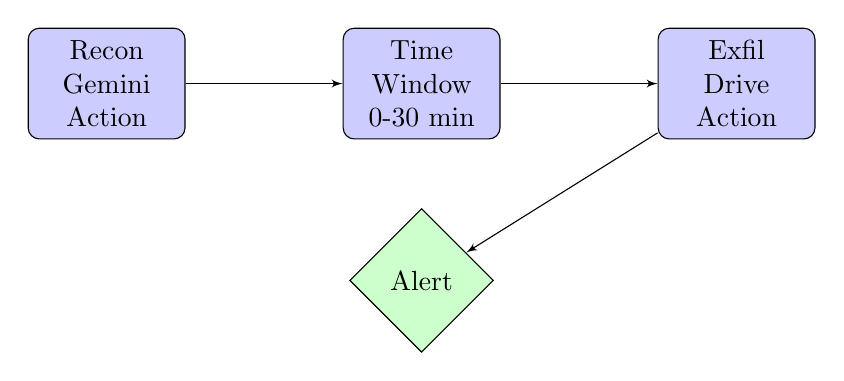
\begin{tikzpicture}[node distance=2cm, auto]
    \tikzstyle{block} = [rectangle, draw, fill=blue!20, 
        text width=5em, text centered, rounded corners, minimum height=4em]
    \tikzstyle{decision} = [diamond, draw, fill=green!20, 
        text width=4.5em, text badly centered, inner sep=0pt]
    \tikzstyle{line} = [draw, -latex']
    
    \node [block] (recon) {Recon\\Gemini Action};
    \node [block, right of=recon, node distance=4cm] (window) {Time Window\\0-30 min};
    \node [block, right of=window, node distance=4cm] (exfil) {Exfil\\Drive Action};
    \node [decision, below of=window, node distance=2.5cm] (alert) {Alert};
    
    \path [line] (recon) -- (window);
    \path [line] (window) -- (exfil);
    \path [line] (exfil) -- (alert);
\end{tikzpicture}
\end{center}

\textbf{Correlation Key:} Actor + Temporal Proximity
\end{frame}

\begin{frame}{Recon Signals (Gemini Events)}
\textbf{Data Source:} Admin SDK Reports API \\
\textbf{Application:} \texttt{gemini\_in\_workspace\_apps} \\
\textbf{Event:} \texttt{feature\_utilization}

\vspace{1em}

\textbf{High-Signal Actions:}
\begin{itemize}
    \item \texttt{ask\_about\_this\_file} - Direct file query
    \item \texttt{summarize\_file} - File summarization
    \item \texttt{analyze\_documents} - Multi-file analysis
    \item \texttt{catch\_me\_up} - Bulk triage
    \item \texttt{report\_unspecified\_files} - Report generation
\end{itemize}

\vspace{1em}

\textbf{Available Since:} 2025-06-20 (180-day retention)
\end{frame}

\begin{frame}{Exfil Signals (Drive Events)}
\textbf{Data Source:} Admin SDK Reports API \\
\textbf{Application:} \texttt{drive}

\vspace{1em}

\textbf{High-Risk Events:}
\begin{itemize}
    \item \texttt{change\_visibility} - Made public/external
    \item \texttt{change\_acl} - External principal added
    \item \texttt{export} - Export to PDF/DOCX/CSV
    \item \texttt{download} - File download
    \item \texttt{copy} - File duplication
    \item \texttt{add\_to\_folder} - Move to external folder
\end{itemize}

\vspace{1em}

\textbf{Key Parameters:} \texttt{doc\_id}, \texttt{visibility}, \texttt{new\_value}, \texttt{old\_value}
\end{frame}

\begin{frame}[fragile]{Detection Algorithm}
\begin{lstlisting}[language=Python]
for exfil_event in drive_events:
    for recon_event in gemini_events:
        if exfil_event.actor == recon_event.actor:
            delta = exfil_event.time - recon_event.time
            
            if 0 <= delta <= 30_minutes:
                severity = calculate_severity(
                    delta, 
                    exfil_event.type,
                    exfil_event.visibility
                )
                
                emit_finding(severity, recon_event, exfil_event)
\end{lstlisting}
\end{frame}

\begin{frame}{Severity Rubric}
\begin{table}
\centering
\small
\begin{tabular}{|l|l|l|}
\hline
\textbf{Severity} & \textbf{Criteria} & \textbf{Response} \\ \hline
High & External share/export $\leq$ 10 min & Page on-call \\ \hline
Medium & External share/export 10-30 min & Next-day review \\ \hline
Low & Any permission change within 30 min & Log for analysis \\ \hline
\end{tabular}
\end{table}

\vspace{1em}

\textbf{Severity Overrides:}
\begin{itemize}
    \item Actor in high-risk OU (Exec, Finance, R\&D) $\rightarrow$ +1 level
    \item File labeled confidential/restricted $\rightarrow$ +1 level
\end{itemize}
\end{frame}

\section{Implementation}

\begin{frame}{Architecture}
\begin{enumerate}
    \item \textbf{Authentication:} Service account with domain-wide delegation
    \item \textbf{Data Collection:} Fetch Gemini + Drive events via Admin SDK
    \item \textbf{Correlation Engine:} Temporal matching by actor
    \item \textbf{Scoring:} Apply severity rules and suppressions
    \item \textbf{Output:} JSON findings to SIEM/alerting
\end{enumerate}

\vspace{1em}

\textbf{Deployment Options:}
\begin{itemize}
    \item Cron job (every 10 minutes)
    \item Systemd timer
    \item Cloud Function / Lambda
\end{itemize}
\end{frame}

\begin{frame}[fragile]{Example Finding (Enhanced)}
\begin{lstlisting}[basicstyle=\ttfamily\tiny]
{
  "severity": "high",
  "actor": "john.doe@company.com",
  "exfil_event": "change_visibility",
  "doc_title": "Q4 Financial Projections.xlsx",
  "delta_minutes": 5.55,
  "reason": "External share within 10min; High recon score (12.5)",
  "recon_score": 12.5,
  "file_context": {
    "sensitivity": "high",
    "labels": ["confidential", "finance"],
    "owner": "cfo@company.com"
  },
  "intent_analysis": {
    "intent": "malicious",
    "confidence": 0.85,
    "reasons": ["Unknown destination domain",
                "Sharing someone else's file",
                "Off-hours activity"],
    "destination_domain": "competitor.com"
  }
}
\end{lstlisting}
\end{frame}

\begin{frame}{Tuning \& Suppression}
\textbf{False Positive Reduction:}
\begin{itemize}
    \item Allowlist trusted external domains (partners)
    \item Suppress security/IT OUs investigating files
    \item Exclude service accounts
    \item Adjust time windows based on your environment
\end{itemize}

\vspace{1em}

\textbf{Calibration Process:}
\begin{enumerate}
    \item Week 1: Observation mode (no alerts)
    \item Week 2: Tune suppressions, enable high severity
    \item Week 3-4: Refinement
    \item Month 2+: Ongoing review
\end{enumerate}
\end{frame}

\section{Results \& Insights}

\begin{frame}{Why This Works}
\textbf{Behavioral Sequence Detection:}
\begin{itemize}
    \item \textbf{Intent:} Gemini logs reveal \textit{what} the user wanted to understand
    \item \textbf{Action:} Drive logs reveal \textit{what} they did with it
    \item \textbf{Correlation:} Temporal proximity reveals insider TTP
\end{itemize}

\vspace{1em}

\textbf{No Content Inspection Required:}
\begin{itemize}
    \item Privacy-preserving detection
    \item No prompt/response content visible
    \item Metadata-only telemetry
\end{itemize}
\end{frame}

\begin{frame}{Detection Advantages}
\begin{columns}[T]
\column{0.5\textwidth}
\textbf{High-Fidelity Signal:}
\begin{itemize}
    \item Precise timestamps
    \item Actor email
    \item File IDs
    \item Action types
\end{itemize}

\column{0.5\textwidth}
\textbf{Google-Recommended:}
\begin{itemize}
    \item Official audit logs
    \item Designed for security telemetry
    \item 180-day retention
    \item No extra cost
\end{itemize}
\end{columns}
\end{frame}

\begin{frame}{Common Patterns Detected}
\begin{enumerate}
    \item \textbf{Rapid Reconnaissance:} User asks Gemini about 10+ files, then downloads 3 with highest value
    \item \textbf{Pre-Resignation Exfil:} Employee uses Gemini to triage entire project folder, then exports key documents
    \item \textbf{Competitive Intelligence:} Sales rep summarizes customer contracts, immediately shares with personal email
    \item \textbf{IP Theft:} Engineer asks Gemini to analyze codebase documentation, then copies to external Git repo
\end{enumerate}
\end{frame}

\section{Operational Considerations}

\begin{frame}{Deployment Checklist}
\begin{enumerate}
    \item Create service account with domain-wide delegation
    \item Grant scopes:
        \begin{itemize}
            \item \texttt{admin.reports.audit.readonly}
            \item \texttt{drive.readonly} (for file context)
        \end{itemize}
    \item Configure Redis for stateful recon tracking (optional)
    \item Configure partner domains \& suppressions
    \item Test with known benign patterns
    \item Start with observation mode (no alerts)
    \item Gradually enable alerting by severity
    \item Integrate with SIEM/SOAR
\end{enumerate}

\vspace{1em}

\textbf{Security Best Practices:}
\begin{itemize}
    \item Store service account key in secrets manager
    \item Rotate keys every 90 days
    \item Monitor the monitor (alert if detector stops)
\end{itemize}
\end{frame}

\begin{frame}{Metrics to Track}
\textbf{Detection Quality:}
\begin{itemize}
    \item True positive rate
    \item False positive rate
    \item Time to detection
    \item Time to response
\end{itemize}

\vspace{1em}

\textbf{Operational:}
\begin{itemize}
    \item Alert volume (findings/day)
    \item API success rate
    \item Coverage (Gemini users / total users)
    \item Alert fatigue score
\end{itemize}
\end{frame}

\begin{frame}{Advanced Features Implemented}
\textbf{Multi-Stage Attack Detection:}
\begin{itemize}
    \item Cumulative recon scoring with 48hr decay half-life
    \item Detects delayed exfil (Day 1: recon, Day 3: exfil)
    \item Redis-backed stateful tracking (with in-memory fallback)
\end{itemize}

\vspace{1em}

\textbf{File Context Enrichment:}
\begin{itemize}
    \item File sensitivity classification (labels, ownership, sharing history)
    \item Automatic severity elevation for confidential files
    \item Workaround for missing doc\_id in Gemini events
\end{itemize}

\vspace{1em}

\textbf{Intent Classification:}
\begin{itemize}
    \item Destination domain reputation (trusted/partner/unknown)
    \item User behavioral baselines (typical sharing patterns)
    \item File ownership checks + off-hours detection
    \item Auto-suppression for legitimate workflows
\end{itemize}
\end{frame}

\begin{frame}{Limitations \& Future Work}
\textbf{Current Limitations:}
\begin{itemize}
    \item Gemini events only since 2025-06-20
    \item 180-day retention window
    \item Gemini API doesn't expose doc\_id (requires heuristics)
    \item Requires Google Workspace Enterprise
\end{itemize}

\vspace{1em}

\textbf{Future Extensions:}
\begin{itemize}
    \item Automated response (revoke links, notify owner)
    \item Integration with HR data (resignations, PIPs)
    \item Cross-correlation with physical security (badge logs)
    \item Bulk recon + mass exfil detection
\end{itemize}
\end{frame}

\section{Conclusion}

\begin{frame}{Key Takeaways}
\begin{enumerate}
    \item \textbf{New Attack Surface:} LLMs enable rapid, efficient insider reconnaissance
    \item \textbf{Behavioral Detection:} Focus on sequences, not content
    \item \textbf{High-Signal:} Temporal correlation of recon + exfil is highly indicative
    \item \textbf{Privacy-Preserving:} No content inspection required
    \item \textbf{Actionable:} Deploy today with Google Admin SDK
\end{enumerate}

\vspace{1em}

\begin{block}{The Bottom Line}
AI-assisted insider threats require AI-aware detection. This technique provides high-fidelity telemetry without compromising user privacy.
\end{block}
\end{frame}

\begin{frame}{Resources}
\textbf{GitHub Repository:} \\
\url{https://github.com/haasonsaas/gemini-exfil-detector}

\vspace{1em}

\textbf{Google Documentation:}
\begin{itemize}
    \item Admin SDK Reports API
    \item Gemini in Workspace Apps Events
    \item Drive Audit Events
\end{itemize}

\vspace{1em}

\textbf{Contact:} \\
GitHub: @haasonsaas

\vspace{1em}

\centering
\Large
\textbf{Questions?}
\end{frame}

\end{document}
